\documentclass[parskip=half,a4paper]{scrartcl}

%%%%%%%%%%%%%%%%%%%%%%%%%%%%%%%%%%%%%%%%%
% Lachaise Assignment
% Structure Specification File
% Version 1.0 (26/6/2018)
%
% This template originates from:
% http://www.LaTeXTemplates.com
%
% Authors:
% Marion Lachaise & François Févotte
% Vel (vel@LaTeXTemplates.com)
%
% License:
% CC BY-NC-SA 3.0 (http://creativecommons.org/licenses/by-nc-sa/3.0/)
%
%%%%%%%%%%%%%%%%%%%%%%%%%%%%%%%%%%%%%%%%%

%----------------------------------------------------------------------------------------
%   PACKAGES AND OTHER DOCUMENT CONFIGURATIONS
%----------------------------------------------------------------------------------------

\usepackage[utf8]{inputenc} % Required for inputting international characters
\usepackage[T1]{fontenc} % Output font encoding for international characters

\usepackage{amsmath,stmaryrd} % Math packages

\usepackage{enumerate} % Custom item numbers for enumerations
\usepackage[shortlabels]{enumitem}
\usepackage{array}
\usepackage{lineno}
\usepackage{epstopdf}
\usepackage{graphics}

\usepackage[ruled]{algorithm2e} % Algorithms

\usepackage[framemethod=tikz]{mdframed} % Allows defining custom boxed/framed environments

\usepackage{minted}

\usepackage[utopia]{mathdesign}
\usepackage{csquotes}

\usepackage{listings} % File listings, with syntax highlighting
\lstset{
    basicstyle=\ttfamily, % Typeset listings in monospace font
    language=Java,
    numbers=left,
    stepnumber=1,
    showstringspaces=false,
    tabsize=3,
    breaklines=true,
    breakatwhitespace=false,
    frame=single,
    linewidth=\columnwidth
}

%----------------------------------------------------------------------------------------
%   DOCUMENT MARGINS
%----------------------------------------------------------------------------------------

\usepackage{geometry} % Required for adjusting page dimensions and margins

\geometry{
    paper=a4paper, % Paper size, change to letterpaper for US letter size
    top=2.5cm, % Top margin
    bottom=3cm, % Bottom margin
    left=2.5cm, % Left margin
    right=2.5cm, % Right margin
    headheight=14pt, % Header height
    footskip=1.5cm, % Space from the bottom margin to the baseline of the footer
    headsep=1.2cm, % Space from the top margin to the baseline of the header
    %showframe, % Uncomment to show how the type block is set on the page
}

%----------------------------------------------------------------------------------------
%   FONTS
%----------------------------------------------------------------------------------------

%----------------------------------------------------------------------------------------
%   COMMAND  ENVIRONMENT
%----------------------------------------------------------------------------------------

% Usage:
% \begin{commandline}
%   \begin{verbatim}
%       $ ls
%
%       Applications    Desktop ...
%   \end{verbatim}
% \end{commandline}

\mdfdefinestyle{commandline}{
    leftmargin=10pt,
    rightmargin=10pt,
    innerleftmargin=15pt,
    middlelinecolor=black!50!white,
    middlelinewidth=2pt,
    frametitlerule=false,
    backgroundcolor=black!5!white,
    frametitle={Command Line},
    frametitlefont={\normalfont\sffamily\color{white}\hspace{-1em}},
    frametitlebackgroundcolor=black!50!white,
    nobreak,
}

% Define a custom environment for command-line snapshots
\newenvironment{commandline}{
    \medskip
    \begin{mdframed}[style=commandline]
}{
    \end{mdframed}
    \medskip
}

%----------------------------------------------------------------------------------------
%   FILE CONTENTS ENVIRONMENT
%----------------------------------------------------------------------------------------

% Usage:
% \begin{file}[optional filename, defaults to "File"]
%   File contents, for example, with a listings environment
% \end{file}

\mdfdefinestyle{file}{
    innertopmargin=1.6\baselineskip,
    innerbottommargin=0.8\baselineskip,
    topline=false, bottomline=false,
    leftline=false, rightline=false,
    leftmargin=2cm,
    rightmargin=2cm,
    singleextra={%
        \draw[fill=black!10!white](P)++(0,-1.2em)rectangle(P-|O);
        \node[anchor=north west]
        at(P-|O){\ttfamily\mdfilename};
        %
        \def\l{3em}
        \draw(O-|P)++(-\l,0)--++(\l,\l)--(P)--(P-|O)--(O)--cycle;
        \draw(O-|P)++(-\l,0)--++(0,\l)--++(\l,0);
    },
    nobreak,
}

% Define a custom environment for file contents
\newenvironment{file}[1][File]{ % Set the default filename to "File"
    \medskip
    \newcommand{\mdfilename}{#1}
    \begin{mdframed}[style=file]
}{
    \end{mdframed}
    \medskip
}

%----------------------------------------------------------------------------------------
%   NUMBERED QUESTIONS ENVIRONMENT
%----------------------------------------------------------------------------------------

% Usage:
% \begin{question}[optional title]
%   Question contents
% \end{question}

\mdfdefinestyle{question}{
    innertopmargin=1.2\baselineskip,
    innerbottommargin=0.8\baselineskip,
    roundcorner=5pt,
    nobreak,
    singleextra={%
        \draw(P-|O)node[xshift=1em,anchor=west,fill=white,draw,rounded corners=5pt]{%
        Question \theQuestion\questionTitle};
    },
}

\newcounter{Question} % Stores the current question number that gets iterated with each new question

% Define a custom environment for numbered questions
\newenvironment{question}[1][\unskip]{
    \bigskip
    \stepcounter{Question}
    \newcommand{\questionTitle}{~#1}
    \begin{mdframed}[style=question]
}{
    \end{mdframed}
    \medskip
}

%----------------------------------------------------------------------------------------
%   WARNING TEXT ENVIRONMENT
%----------------------------------------------------------------------------------------

% Usage:
% \begin{warn}[optional title, defaults to "Warning:"]
%   Contents
% \end{warn}

\mdfdefinestyle{warning}{
    topline=false, bottomline=false,
    leftline=false, rightline=false,
    nobreak,
    singleextra={%
        \draw(P-|O)++(-0.5em,0)node(tmp1){};
        \draw(P-|O)++(0.5em,0)node(tmp2){};
        \fill[black,rotate around={45:(P-|O)}](tmp1)rectangle(tmp2);
        \node at(P-|O){\color{white}\scriptsize\bf !};
        \draw[very thick](P-|O)++(0,-1em)--(O);%--(O-|P);
    }
}

% Define a custom environment for warning text
\newenvironment{warn}[1][Warning:]{ % Set the default warning to "Warning:"
    \medskip
    \begin{mdframed}[style=warning]
        \noindent{\textbf{#1}}
}{
    \end{mdframed}
}

%----------------------------------------------------------------------------------------
%   INFORMATION ENVIRONMENT
%----------------------------------------------------------------------------------------

% Usage:
% \begin{info}[optional title, defaults to "Info:"]
%   contents
%   \end{info}

\mdfdefinestyle{info}{%
    topline=false, bottomline=false,
    leftline=false, rightline=false,
    nobreak,
    singleextra={%
        \fill[black](P-|O)circle[radius=0.4em];
        \node at(P-|O){\color{white}\scriptsize\bf i};
        \draw[very thick](P-|O)++(0,-0.8em)--(O);%--(O-|P);
    }
}

% Define a custom environment for information
\newenvironment{info}[1][Info:]{ % Set the default title to "Info:"
    \medskip
    \begin{mdframed}[style=info]
        \noindent{\textbf{#1}}
}{
    \end{mdframed}
}


\newdimen\longformulasindent
\newenvironment{longformulas}
 {\global\longformulasindent=0pt
  \def\>{\global\advance\longformulasindent2em\relax\hspace{2em}}%
  \def\<{\global\advance\longformulasindent-2em\relax\hspace{-2em}}%
  \renewcommand{\arraystretch}{1.2}% some more room
  \begin{array}{@{}>{\displaystyle\hspace{\longformulasindent}}l@{}}}
 {\end{array}}

\newcommand{\code}{\texttt}


\title{Machine Learning Excercise 1}
\author{Laszlo Korte, MtrNr. 6329857}
\date{Universität Hamburg --- \today}

\begin{document}

\maketitle


\section*{Hypothesis}

The goal is to find a polynomial to aproximate our data points. We know that the source of our data points is one period of the sine function. One sine period has one maximum and one minumum. So we can presume that a polynomial of degree 3 is sufficent to fit our points.

$$
y = f(x) =
  \theta_0
+ \theta_1 x
+ \theta_2 x^2
+ \theta_3 x^3
$$


\section*{Result}

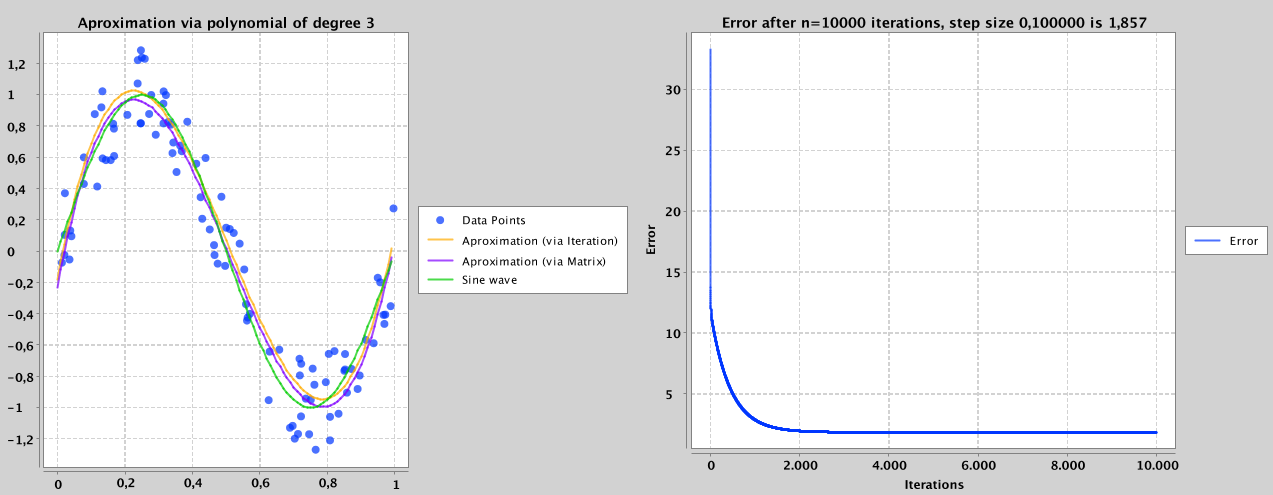
\includegraphics[width=\textwidth]{fig3.png}

The polynomial

$$
f(x) = \begin{bmatrix}
-0.18389300723650462 \\
11.861463633653237 \\
-33.86021075015673 \\
22.307252966654328
\end{bmatrix}^T
\begin{bmatrix}
x^0 \\
x^1 \\
x^2 \\
x^3 \\
\end{bmatrix}
$$

has been computed using stochastic gradient descent algorithm using a learning rate of $\alpha = 0.2$ yielding a final error of $1.857$


\section*{Optimizing the learnign rate}

Using the gradient gradient descent algorithm with learning rate $\alpha = 0.001$ and wating for a maximum of 10.000 iterations we get

$$
\theta = \begin{bmatrix}
0.5836921783142958,
0.13027164529834673,
-4.315198280227572,
2.746957039499795
\end{bmatrix}
$$

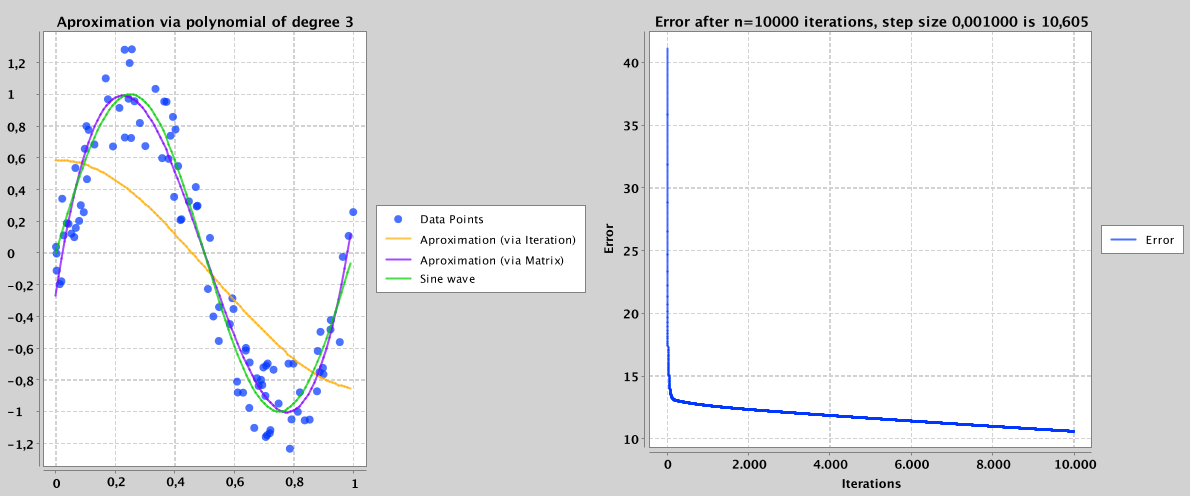
\includegraphics[width=\textwidth]{fig1.png}

But as we can see the resulting curve does not really fit the points and the final error is above $>10$. Plotting the error we see that indeed it decreases with each iteration and would decrease further if we allow the algorithm to iterate further. But the slope of the error plot is already getting pretty low and we do not want to wait much longer for the error to decrease.

Instead of increasing the maximum iterations we try to increase the learning rate $\alpha$ to let the algorithm progress faster.

Using the gradient gradient descent algorithm with learning rate $\alpha = 0.01$ and wating for a maximum of 10.000 iterations we get

$$
\theta = \begin{bmatrix}
0.2124157957316986,
7.179268724738586,
-23.335012658458066,
15.78218638956732
\end{bmatrix}
$$

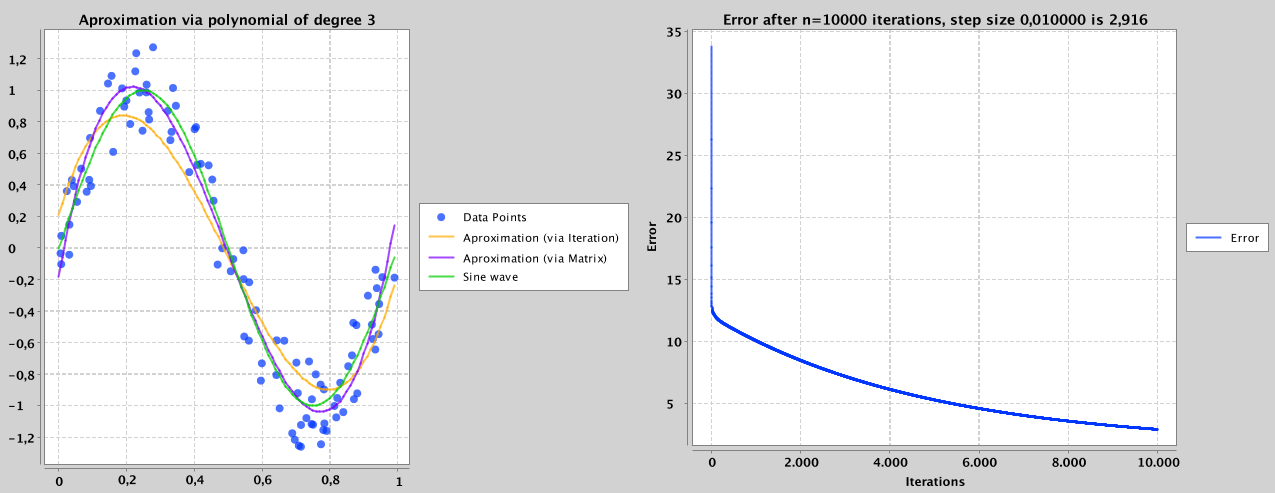
\includegraphics[width=\textwidth]{fig2.png}

Plotting the polynom we can see it fits the points much better. Plotting the error we can see that it's dropping much faster below $10$ and just below $3$ after the same number of iterations as before. Ee can also see that increasing the number of iterations would further decrease the error. But instead we further increase the learning rate.

Using the gradient gradient descent algorithm with learning rate $\alpha = 0.0$ and wating for a maximum of 10.000 iterations we get


$$
\theta = \begin{bmatrix}
-0.18389300723650462,
11.861463633653237,
-33.86021075015673,
22.307252966654328
\end{bmatrix}
$$

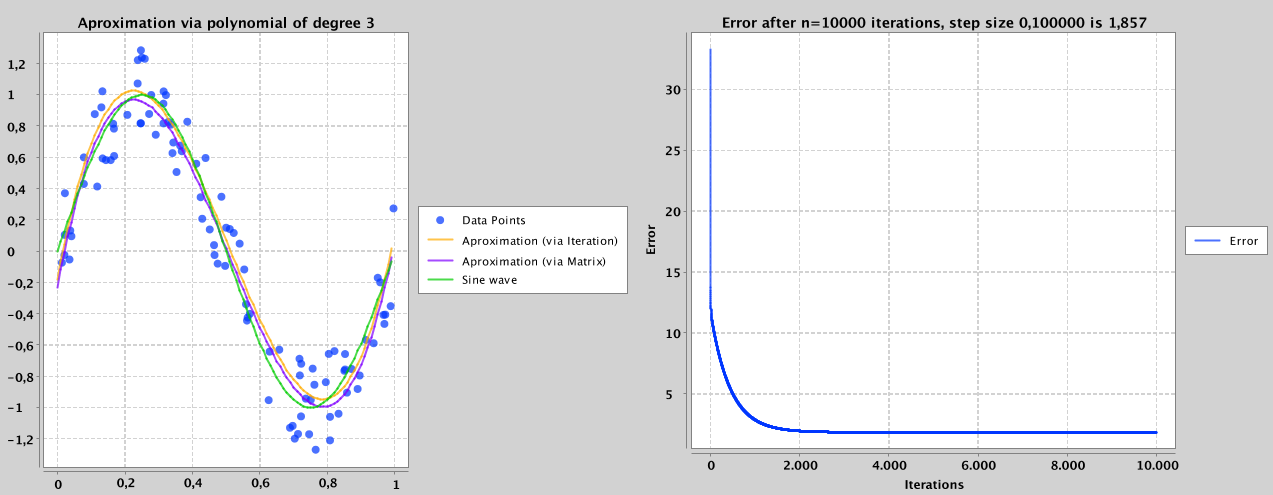
\includegraphics[width=\textwidth]{fig3.png}


Now the function fits the points pretty well and plotting the error we can see that it already converges after 4000 iterations at about $1.8$.

Increasing the learning rate to much also increases the final error again. We could now do for example a binary search for the optimal learning rate and then increase the iterations until we are satisfied with a low low enough final error.

But just looking at the plot of the function matching the points we can already settle for the polynomial

$$
f(x) = \begin{bmatrix}
-0.18389300723650462\\
11.861463633653237\\
-33.86021075015673\\
22.307252966654328
\end{bmatrix}^T
\begin{bmatrix}
x^0 \\
x^1 \\
x^2 \\
x^3 \\
\end{bmatrix}
$$

and an error of $1.857$

\pagebreak

\section*{Implementation}

\begin{minted}{clojure}

(defn build-polynomial [pairs degree]
  "convert [x y] pairs into {:x :y} map where"
  ":x becomes a vector of powers of x"
  (->> pairs
       (map
        (fn [[x y]] {:x (powers x degree)
                     :y y}))
       (vec)))

(defn gradient-descent [data alpha theta]
  "gradient descent algorithm"
  "alpha is the the learning rate"
  "theta is the initial vector of coefficients"
  (->> data
       (reduce
        (fn [t d]
          (m/add-scaled t
                        (:x d)
                        (* alpha
                           (- (:y d)
                              (m/dot t (:x d))))))
        theta)))

(defn find-polynomial [points degree learning-rate]
  "given a list of points find a polynomial of degree"
  "using gradient descent algorithm with learning-rate"
  (let [data (build-polynomial points degree)]
    (->> #(noise 0.5)
         ; initialize coefficients
         (repeatedly)
         (take (inc degree))
         (vec)
         ; apply gradient descent
         (iterate #(gradient-descent data learning-rate %1)))
\end{minted}



\end{document}
